%!TEX root = ../TAMUTemplate.tex
%%%%%%%%%%%%%%%%%%%%%%%%%%%%%%%%%%%%%%%%%%%%%%%%%%%
%
%  New template code for TAMU Theses and Dissertations starting Fall 2016.
%
%  Author: Sean Zachary Roberson
%	 Version 3.16.09
%  Last updated 9/12/2016
%
%%%%%%%%%%%%%%%%%%%%%%%%%%%%%%%%%%%%%%%%%%%%%%%%%%%
%%%%%%%%%%%%%%%%%%%%%%%%%%%%%%%%%%%%%%%%%%%%%%%%%%%%%%%%%%%%%%%%%%%%%%
%%                           SECTION VI
%%%%%%%%%%%%%%%%%%%%%%%%%%%%%%%%%%%%%%%%%%%%%%%%%%%%%%%%%%%%%%%%%%%%%


\chapter{\texorpdfstring{\uppercase {Results}}{Results}}
\label{ch:results}

The KinMEBDT distributions showing the background predictions and the observed data are shown in fig.~\ref{fig:KinMEBDT_final_templates}.
The Higgs signal hypothesis with \joinsym{\MH}{=}{125\gev} is enlarged and shown using a red line to indicate where in the distribution the signal would lie.
There is good agreement between the observed data and simulated background estimate; certainly well withing the systematic errors shown using the gray hashed areas.
These distributions contain one histogram for each signal, background, and data sample.
These template histograms are used as the input for our shape based limit setting procedure, each bin acting as a counting experiment, but with correlated systematics.

\begin{figure}[!hbtp]
    \centering
    \begin{subfigure}[t]{0.316\textwidth}
        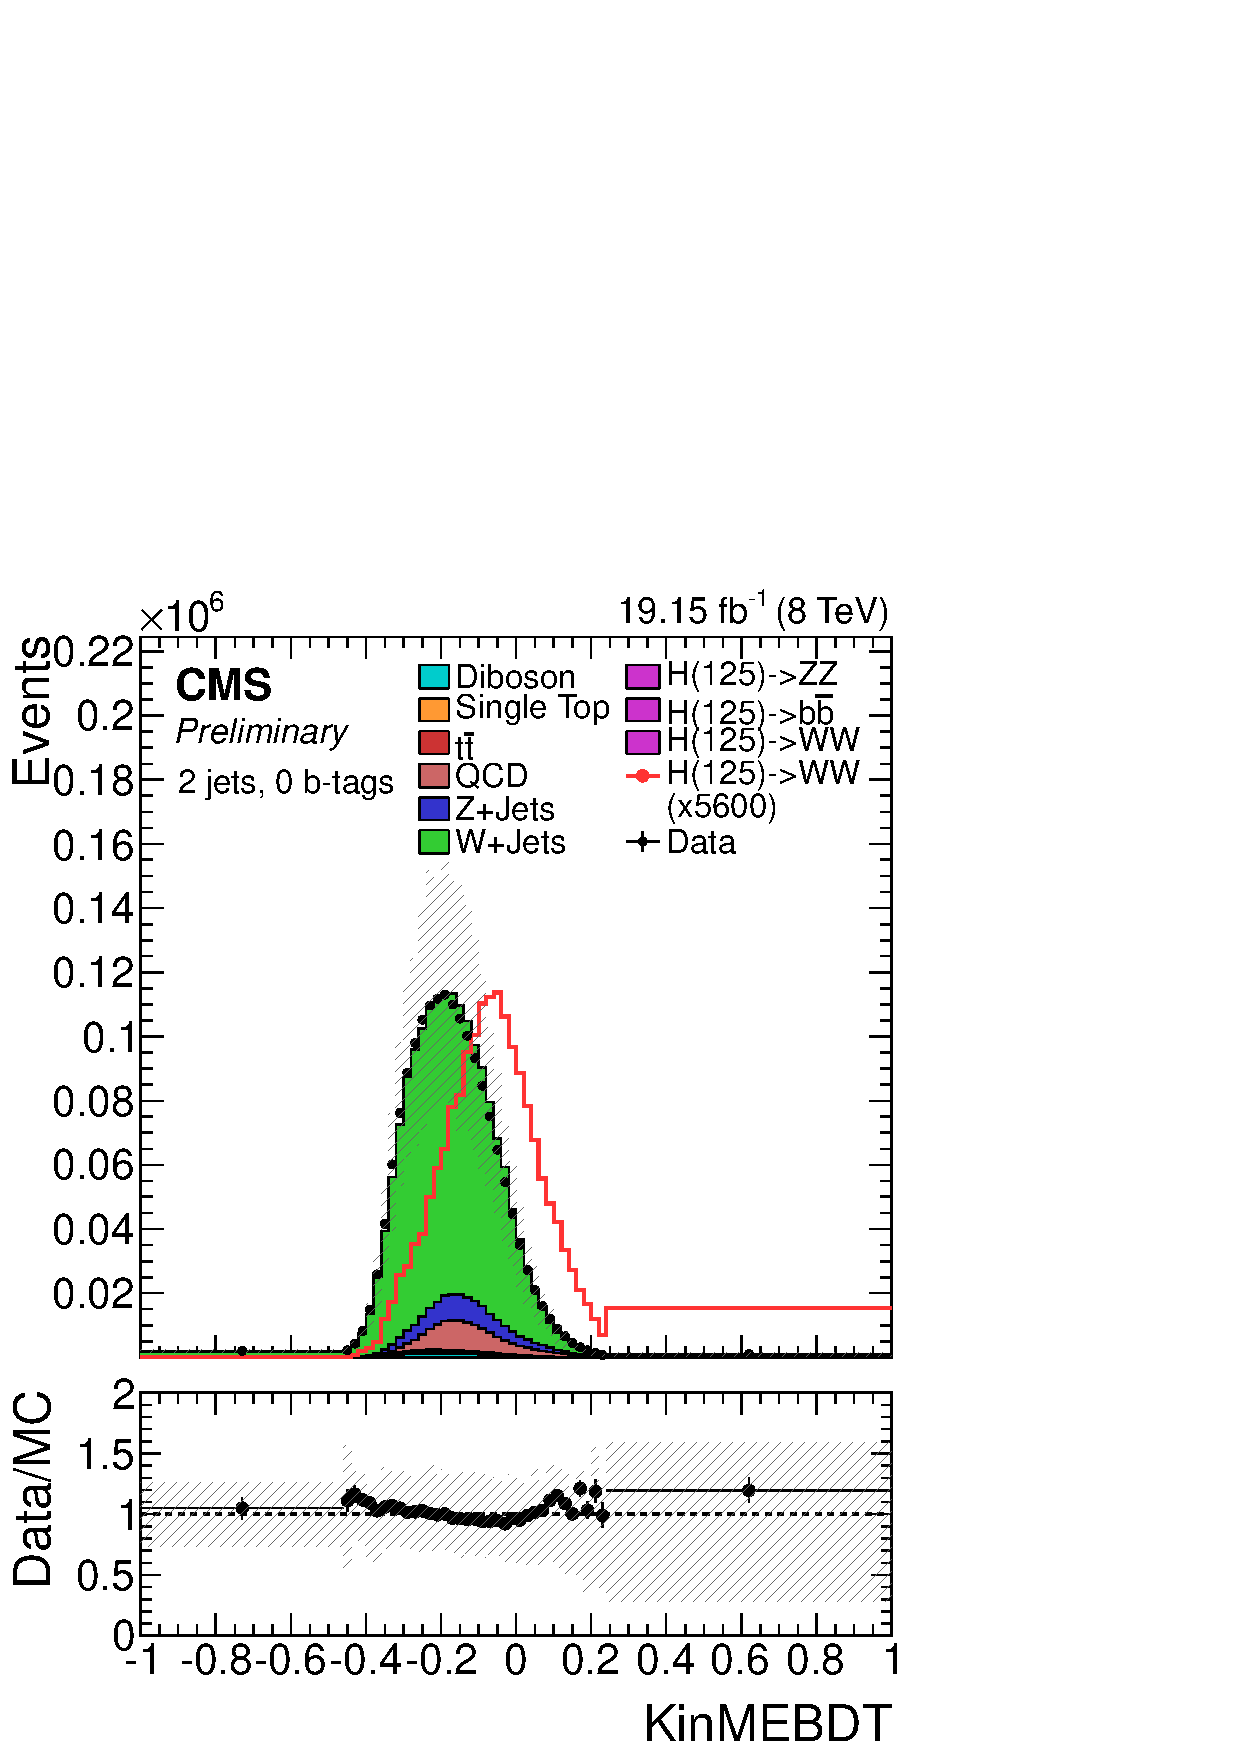
\includegraphics[width=\textwidth]{\figpath/Chapter6/KinMEBDT_jets2_electron.png}
        \caption{}
        \label{fig:KinMEBDT_jets2_electron}
    \end{subfigure}
    \begin{subfigure}[t]{0.316\textwidth}
        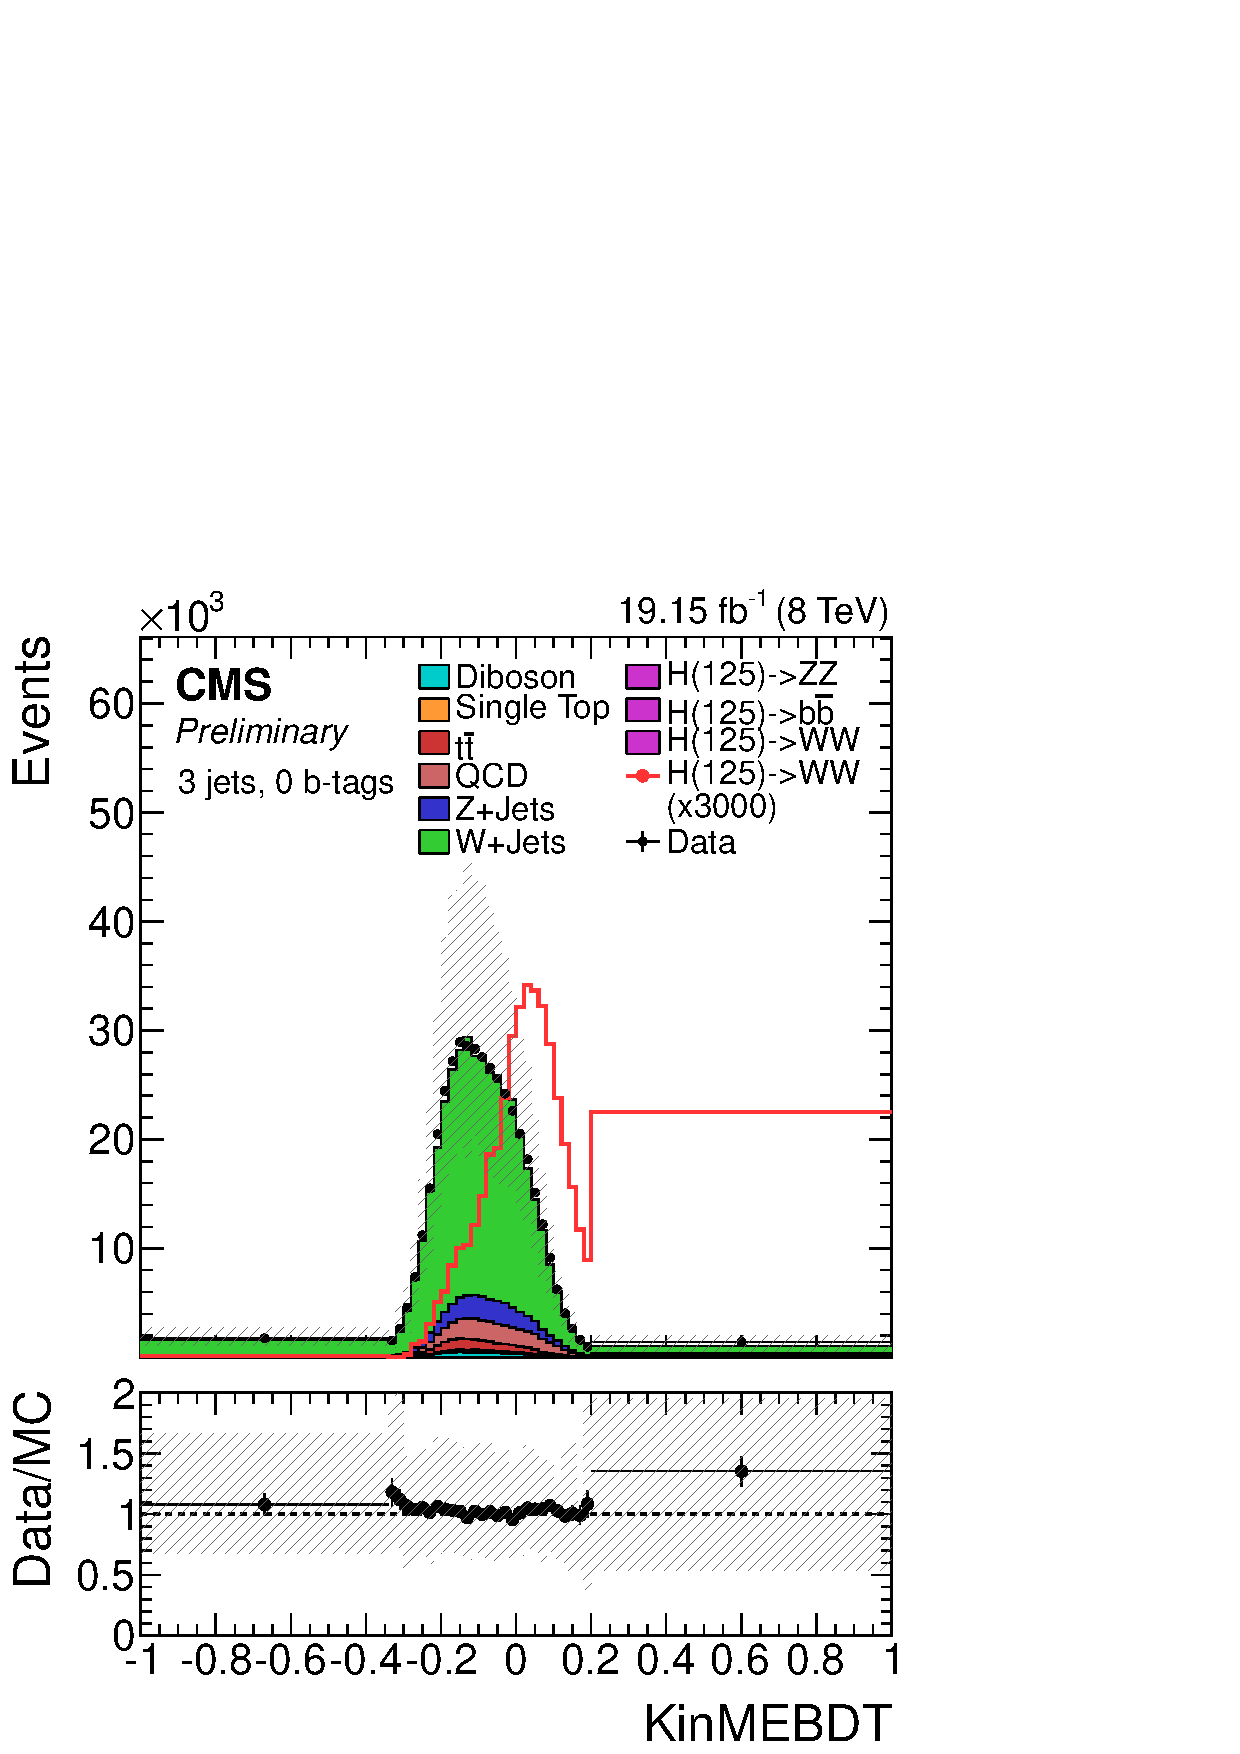
\includegraphics[width=\textwidth]{\figpath/Chapter6/KinMEBDT_jets3_electron.png}
        \caption{}
        \label{fig:KinMEBDT_jets3_electron}
    \end{subfigure}
    \begin{subfigure}[t]{0.316\textwidth}
        \includegraphics[width=\textwidth]{\figpath/Chapter6/KinMEBDT_jets4_electron.png}
        \caption{}
        \label{fig:KinMEBDT_jets4_electron}
    \end{subfigure}

    \begin{subfigure}[t]{0.316\textwidth}
        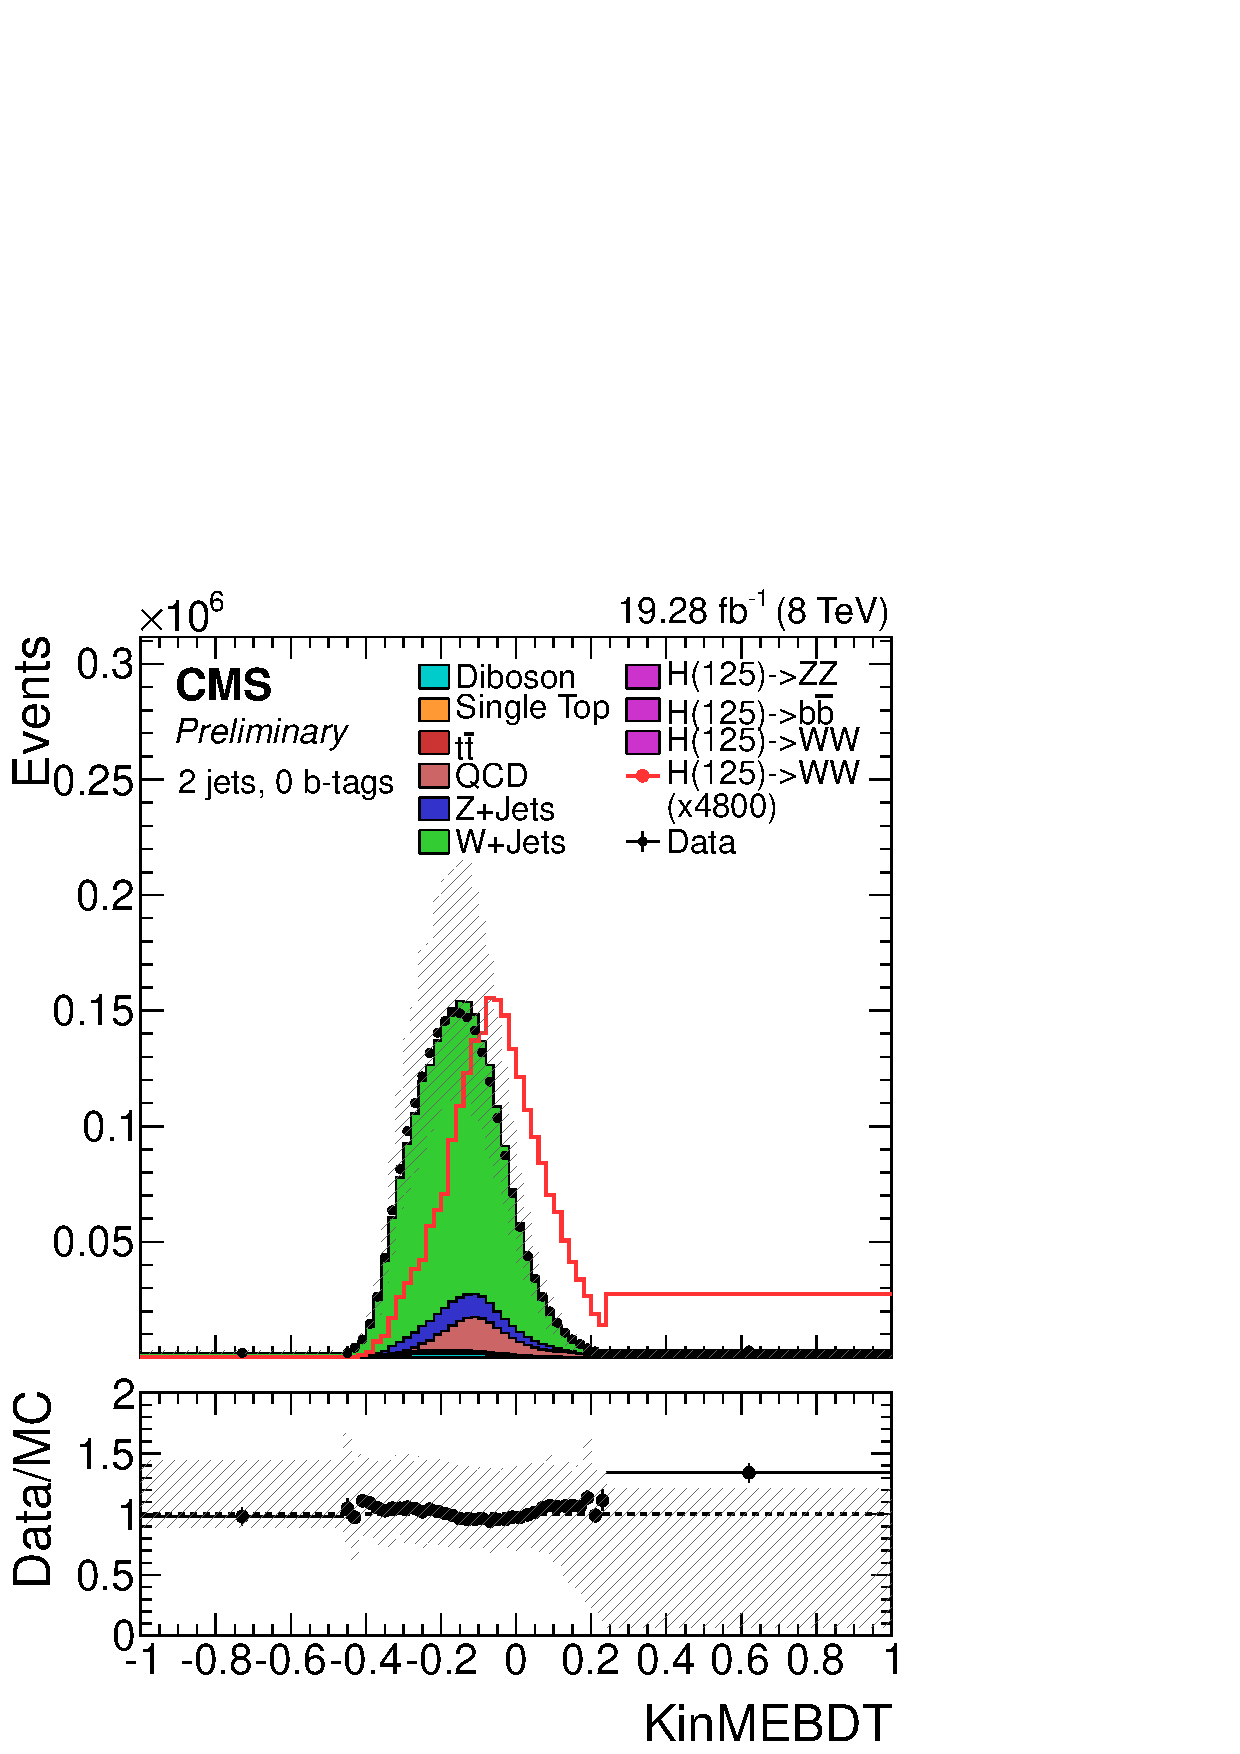
\includegraphics[width=\textwidth]{\figpath/Chapter6/KinMEBDT_jets2_muon.png}
        \caption{}
        \label{fig:KinMEBDT_jets2_muon}
    \end{subfigure}
    \begin{subfigure}[t]{0.316\textwidth}
        \includegraphics[width=\textwidth]{\figpath/Chapter6/KinMEBDT_jets3_muon.png}
        \caption{}
        \label{fig:KinMEBDT_jets3_muon}
    \end{subfigure}
    \begin{subfigure}[t]{0.316\textwidth}
        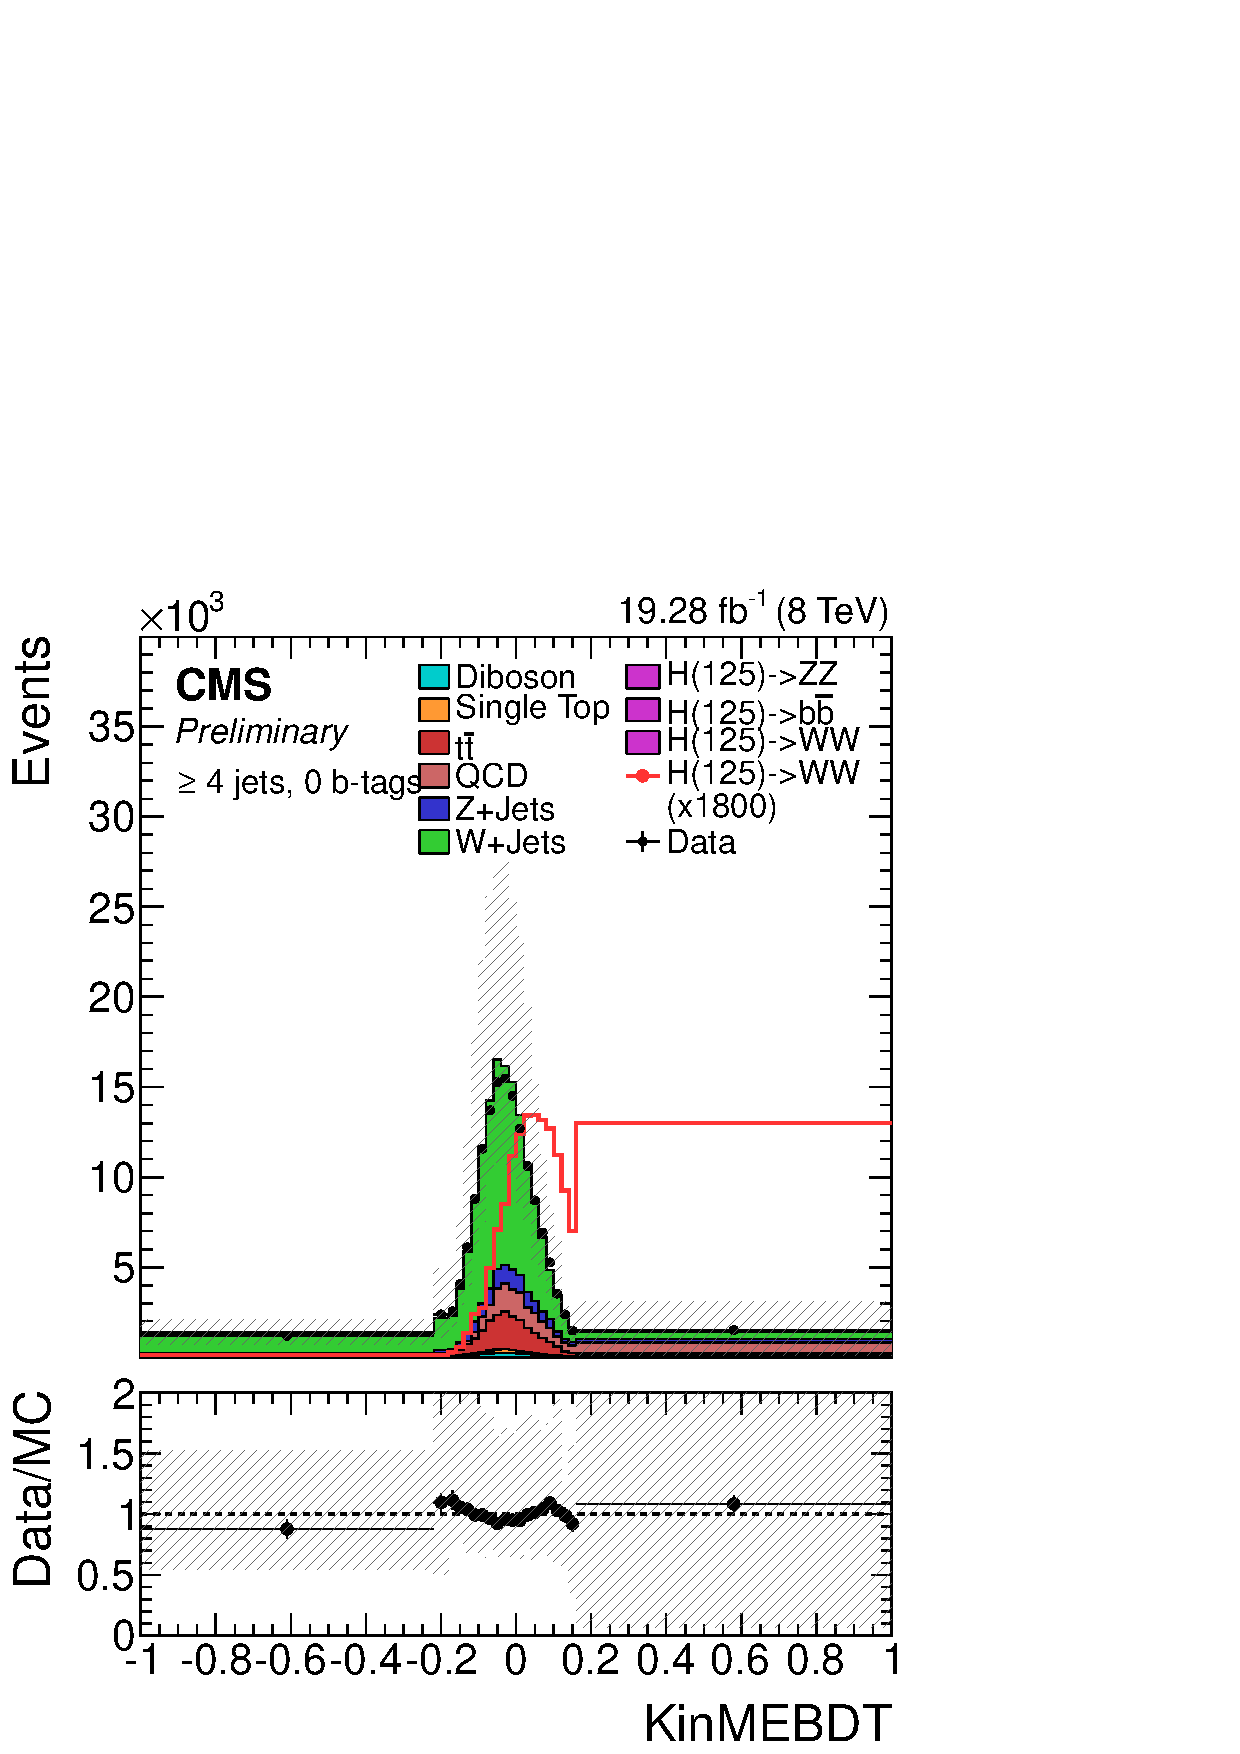
\includegraphics[width=\textwidth]{\figpath/Chapter6/KinMEBDT_jets4_muon.png}
        \caption{}
        \label{fig:KinMEBDT_jets4_muon}
    \end{subfigure}
    \caption{The KinMEBDT distribution in Monte Carlo (filled histograms) and data (black markers). The \HWW signal is shown by red line while the systematic uncertainties are shown by the hashed areas. The plots are ordered by jet bin from left to right, with the leftmost plot being the two-jet bin and the rightmost plot being the greater than or equal to four-jet bin. The top row contains the electron channel plots while the bottom rows contain the muon channel plots.}
    \label{fig:KinMEBDT_final_templates}
\end{figure}

Because no significant excess of signal events was observed, the best we can do is set an upper limit on the production cross sections of \HWWlvjj.
The results are reported as an upper bound on $\sigma/\sigma_{\text{SM}}$ at the 95\% confidence level (CL), made by using the modified-frequentist limit setting method with the CL\textsubscript{S} test statistic~\cite{Read:presentation,Junk,LHC-HCG}.
Although it is more rigorous to use the toy-based frequentist limit setting procedures, these methods are known to take an exceedingly long time to converge.
However, when not in a low statistics regime, the toy-based methods and the asymptotic approximation return roughly equivalent answers.
Therefore, we used the asymptotic approximation as we do indeed have copious amounts of background and data in our templates.
The computations were done using the Higgs Combine Tool~\cite{HiggsCombineTwiki}, which is a RooStats~\cite{Schott:2012zb} based limit setting package.
Appendix~\ref{appendix:limit_setting} contains a more detailed discussion on the computation of the CL\textsubscript{S} limits.
The expected and observed upper limits on $\sigma/\sigma_{\text{SM}}$ are shown in fig.~\ref{fig:limits_withSys_muon}, with the actual values listed in table~\ref{tab:95percent_upper_confidence_levels}.

\begin{comment}
Rishi:
The p-value of the excess at 125 GeV is 3.2σ.

To quantify, how probable the observed excess of events is above the background fluctuations the combined p-value is computed for the best-fit Higgs mass of 124.7GeV with a statistical significance of 5.65σ
\end{comment}

\begin{figure}[!hbt]
    \centering
    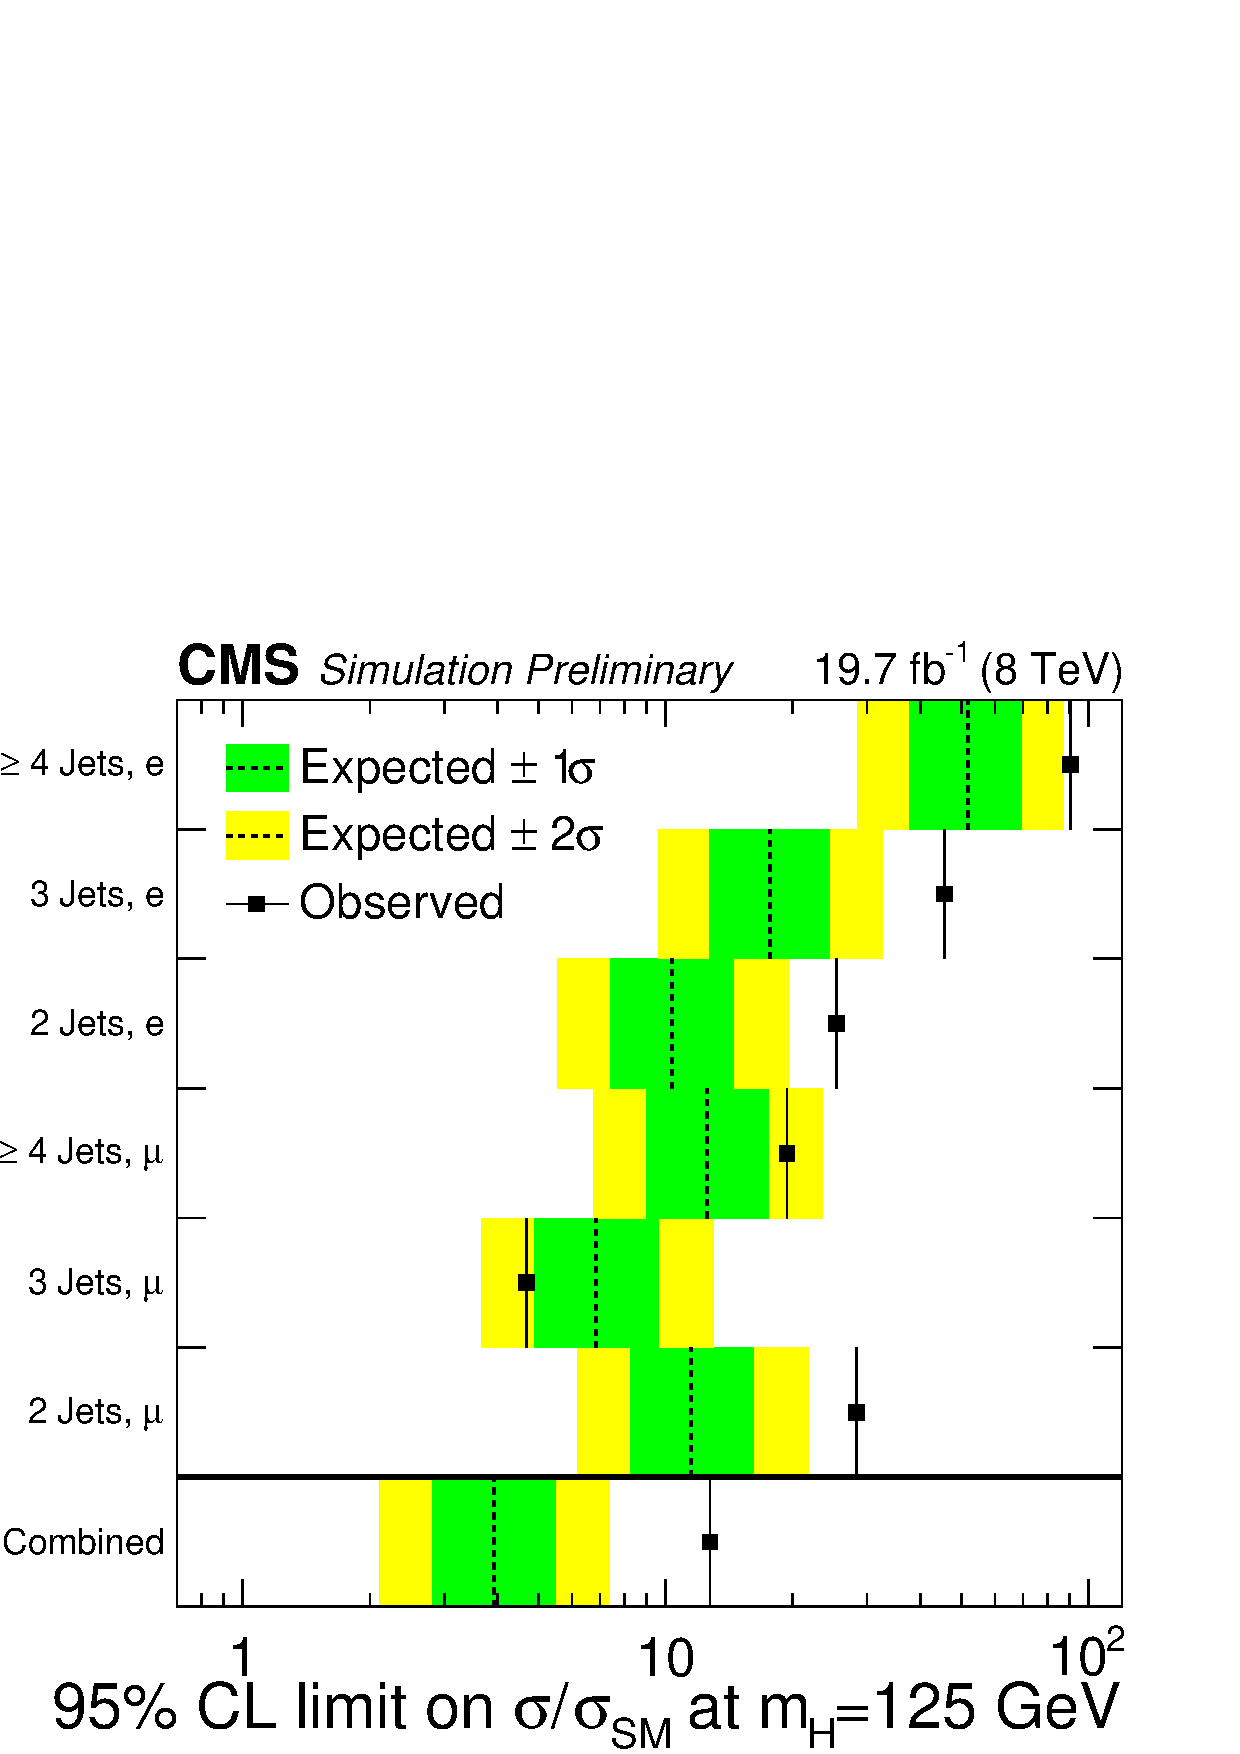
\includegraphics[width=0.95\textwidth]{\figpath/Chapter6/2017_11_13_combinedSM_KinMEBDT.pdf}
    \caption{Median expected and observed 95\% upper confidence level on the cross-section ratio to the expected Standard Model Higgs cross-section ($\mu$) for only the muon channel. The green and yellow uncertainty bands represent the 68\% and 95\% CL intervals on the expected limit, respectively. The values were found using the Asymptotic CL\textsubscript{S} approximation.}
    \label{fig:limits_withSys_muon}
\end{figure}

\begin{table}[htbp]
\centering
\begin{tabular}{lrr} \hline
Category                            & Observed & Expected               \\
\hline\\[-2.45ex]
$\geqslant$4 Jets (\Pe)             & $90.6$   & $51.9_{-14.1}^{+17.6}$ \\
3 Jets (\Pe)                        & $45.6$   & $17.7_{-5.0}^{+6.7}$   \\
2 Jets (\Pe)                        & $25.4$   & $10.3_{-2.9}^{+4.2}$   \\
$\geqslant$4 Jets (\Pmu)            & $19.4$   & $12.6_{-3.6}^{+5.0}$   \\
3 Jets (\Pmu)                       & $4.7$    & $6.8_{-1.9}^{+2.8}$    \\
2 Jets (\Pmu)                       & $28.2$   & $11.5_{-3.3}^{+4.6}$   \\
\hline\\[-2.45ex]
%2 Jets (Combined Lepton)            &          & $7.2_{-5.2}^{+10.0}$  \\
%3 Jets (Combined Lepton)            &          & $4.7_{-3.4}^{+6.6}$   \\
%$\geqslant$4 Jets (Combined Lepton) &          & $8.2_{-5.8}^{+11.4}$  \\
%\hline\\[-2.45ex]
%Combined Jets (\Pe)                 &          & $4.0_{-1.1}^{+1.6}$   \\
%Combined Jets (\Pmu)                & $4.1$    & $5.4_{-1.5}^{+2.2}$   \\
%\hline\\[-2.45ex]
Combined                            & 12.7      & $3.9_{-1.1}^{+1.6}$   \\
%Significance: 4.08718
%       (p-value = 2.1832e-05)
\hline
\end{tabular}
\caption{Observed and median expected and 95\% CLs upper limits on $\mu$ calculated with the Asymptotic CL\textsubscript{S} method. The $\pm1\sigma$ confidence interval is quoted for the expected limits.}
\label{tab:95percent_upper_confidence_levels}
\end{table}